\section{Results}

\subsection{The Corroborated Evidence Base}
Table~\ref{tab:t4} lists every outcome record carried into the synthesis, with its sensing
configuration, evaluation data, cohort size, validation protocol, metric and value. Across
the 29 accuracy records the median is $93.00\%$ with an interquartile range of
$87.37$ to $96.09\%$. Two features of the table are more informative than that central
tendency. First, the protocol column is dominated by \textit{Not reported}: only 8 of the 60
included studies state a validation protocol recoverably, so for most records it cannot be
determined whether the reported number reflects subject-dependent or subject-independent
performance. Second, the highest values in the table belong to unimodal systems. Blood volume
pulse alone reaches $98.23\%$ on WESAD \cite{r50}, and in-ear PPG alone reaches $97.78\%$
\cite{r43}, both above every multimodal record in the table. This is already inconsistent
with a strong reading of the fusion hypothesis.

\begin{table}[!htbp]
\centering
\caption{Corroborated outcome records contributing to the quantitative synthesis. Every value
was recovered from the publisher or indexed record; no value is taken from a secondary
citation. LOSO denotes leave-one-subject-out validation and NR denotes a cohort size or
protocol that could not be recovered.}
\label{tab:t4}
\scriptsize
\resizebox{\textwidth}{!}{\begin{tabular}{L{2.8cm} C{0.7cm} L{3.2cm} L{2.45cm} C{0.7cm} L{1.8cm} C{0.9cm} C{1.1cm}}
\toprule
\textbf{Study} & \textbf{Year} & \textbf{Sensing configuration} & \textbf{Evaluation data} & \textbf{$n$} & \textbf{Protocol} & \textbf{Metric} & \textbf{Value (\%)} \\
\midrule
Abdul Kader et al. \cite{r75} & 2024 & EEG+GSR & In-house & 20 & Not reported & Accuracy & 84.60 \\
Ali et al. (ReTeNet) \cite{r50} & 2025 & BVP & WESAD & 15 & Not reported & Accuracy & 98.23 \\
Ali et al. (SADDNet) \cite{r47} & 2026 & PPG & CATSA+WESAD & 50 & LOSO & Accuracy & 92.25 \\
Ali et al. (TEANet) \cite{r55} & 2026 & BVP & WESAD & 15 & LOSO & Accuracy & 96.94 \\
Ali et al. (TEANet) \cite{r55} & 2026 & BVP & RUET-SPML & 19 & LOSO & Accuracy & 92.94 \\
Alsahreef et al. \cite{r1} & 2026 & HRV & PARFAIT & NR & Not reported & Accuracy & 98.10 \\
Awada et al. \cite{r26} & 2024 & EDA+BVP+TEMP+behav. & In-house (office) & NR & Not reported & Accuracy & 82.78 \\
Barki et al. \cite{r43} & 2025 & In-ear PPG & In-house & 15 & Not reported & Accuracy & 97.78 \\
Campanella et al. \cite{r12} & 2023 & PPG+EDA & In-house & 29 & Not reported & Accuracy & 90.00 \\
Chen \& Lee \cite{r74} & 2023 & ECG & In-house & NR & Not reported & Accuracy & 93.42 \\
Donati et al. \cite{r5} & 2023 & ECG & In-house (factory) & NR & Not reported & Accuracy & 88.40 \\
El Arwadi \& Abu Daher \cite{r21} & 2025 & ECG (HRV) & In-house & NR & LOSO & Accuracy & 90.80 \\
Fernandez et al. \cite{r30} & 2025 & EEG & In-house & NR & Subject indep. & Accuracy & 86.24 \\
Gedam et al. \cite{r99} & 2025 & ECG+GSR+TEMP & In-house & 200 & Not reported & Accuracy & 96.17 \\
Hongn et al. \cite{r19} & 2025 & EDA+BVP+TEMP+ACC & In-house (public) & 36 & Not reported & Accuracy & 93.00 \\
Khayyat et al. \cite{r61} & 2024 & HRV & WESAD & 15 & Not reported & Accuracy & 96.76 \\
Khayyat et al. \cite{r61} & 2024 & HRV & SWELL-KW & 25 & Not reported & Accuracy & 92.76 \\
Kim et al. \cite{r37} & 2024 & EEG+GSR & In-house (VR interview) & 30 & Not reported & AUROC & 95.40 \\
Kim et al. \cite{r109} & 2025 & HR+step count & In-house (free living) & NR & Not reported & Accuracy & 74.40 \\
Kumar et al. \cite{r25} & 2024 & PPG+EDA+TEMP & In-house & NR & Not reported & Accuracy & 94.00 \\
Laiti et al. \cite{r49} & 2026 & PPG (HRV) & WESAD & 15 & Not reported & AUROC & 91.58 \\
Laiti et al. \cite{r49} & 2026 & PPG (HRV) & Wellby (real world) & NR & Not reported & AUROC & 77.02 \\
Li \& Washington \cite{r33} & 2024 & BVP+EDA+TEMP & WESAD & 15 & Personalized & Accuracy & 95.06 \\
Li \& Washington \cite{r33} & 2024 & BVP+EDA+TEMP & WESAD & 15 & Subject indep. & Accuracy & 67.65 \\
Mohammadi et al. \cite{r14} & 2022 & ECG+EDA+RESP+TEMP & WESAD & 15 & Not reported & Accuracy & 96.00 \\
Momeni et al. \cite{r54} & 2022 & ECG+EDA+RESP+TEMP & In-house & NR & Not reported & Accuracy & 90.98 \\
Rashid et al. \cite{r58} & 2023 & BVP+EDA+TEMP+ACC & WESAD & 15 & Not reported & Accuracy & 94.12 \\
Rashid et al. \cite{r58} & 2023 & BVP+EDA+TEMP+ACC & WESAD & 15 & Not reported & Accuracy & 86.34 \\
Rescio et al. \cite{r4} & 2024 & EEG+ECG+EDA & In-house & NR & Not reported & Accuracy & 95.38 \\
Shikha et al. \cite{r53} & 2024 & EDA+BVP+HRV & In-house & NR & Not reported & Accuracy & 98.28 \\
Toshnazarov et al. \cite{r13} & 2024 & PPG+ACC+context & In-house (lab) & 26 & Not reported & F1 & 84.00 \\
Toshnazarov et al. \cite{r13} & 2024 & PPG+ACC+context & In-house (field) & 18 & Not reported & F1 & 71.00 \\
Xu et al. \cite{r16} & 2024 & Facial video (rPPG) & In-house & NR & Not reported & Accuracy & 94.33 \\
Xu et al. \cite{r16} & 2024 & Facial video (rPPG) & In-house & NR & Not reported & Accuracy & 83.83 \\
\midrule
\multicolumn{7}{l}{\textbf{Median corroborated accuracy across 29 accuracy records}} & \textbf{93.00} \\
\multicolumn{7}{l}{Interquartile range} & 87.37--96.09 \\
\bottomrule
\end{tabular}}
\end{table}

Figure~\ref{fig:modality} groups the corroborated accuracy records by sensing configuration.
Median accuracy for single-channel PPG, BVP or ECG systems is close to that of configurations
combining three or more physiological channels, and the camera-based records sit within the
same band. The distributions overlap almost completely. Because these are between-study
comparisons they cannot support a causal claim in either direction, which is precisely why
the analysis in Sections~4.3 and~4.4 is restricted to within-study contrasts; what
Figure~\ref{fig:modality} does establish is that the between-study evidence conventionally
cited in support of fusion contains no visible modality effect to begin with.

\begin{figure}[!htbp]
\centering
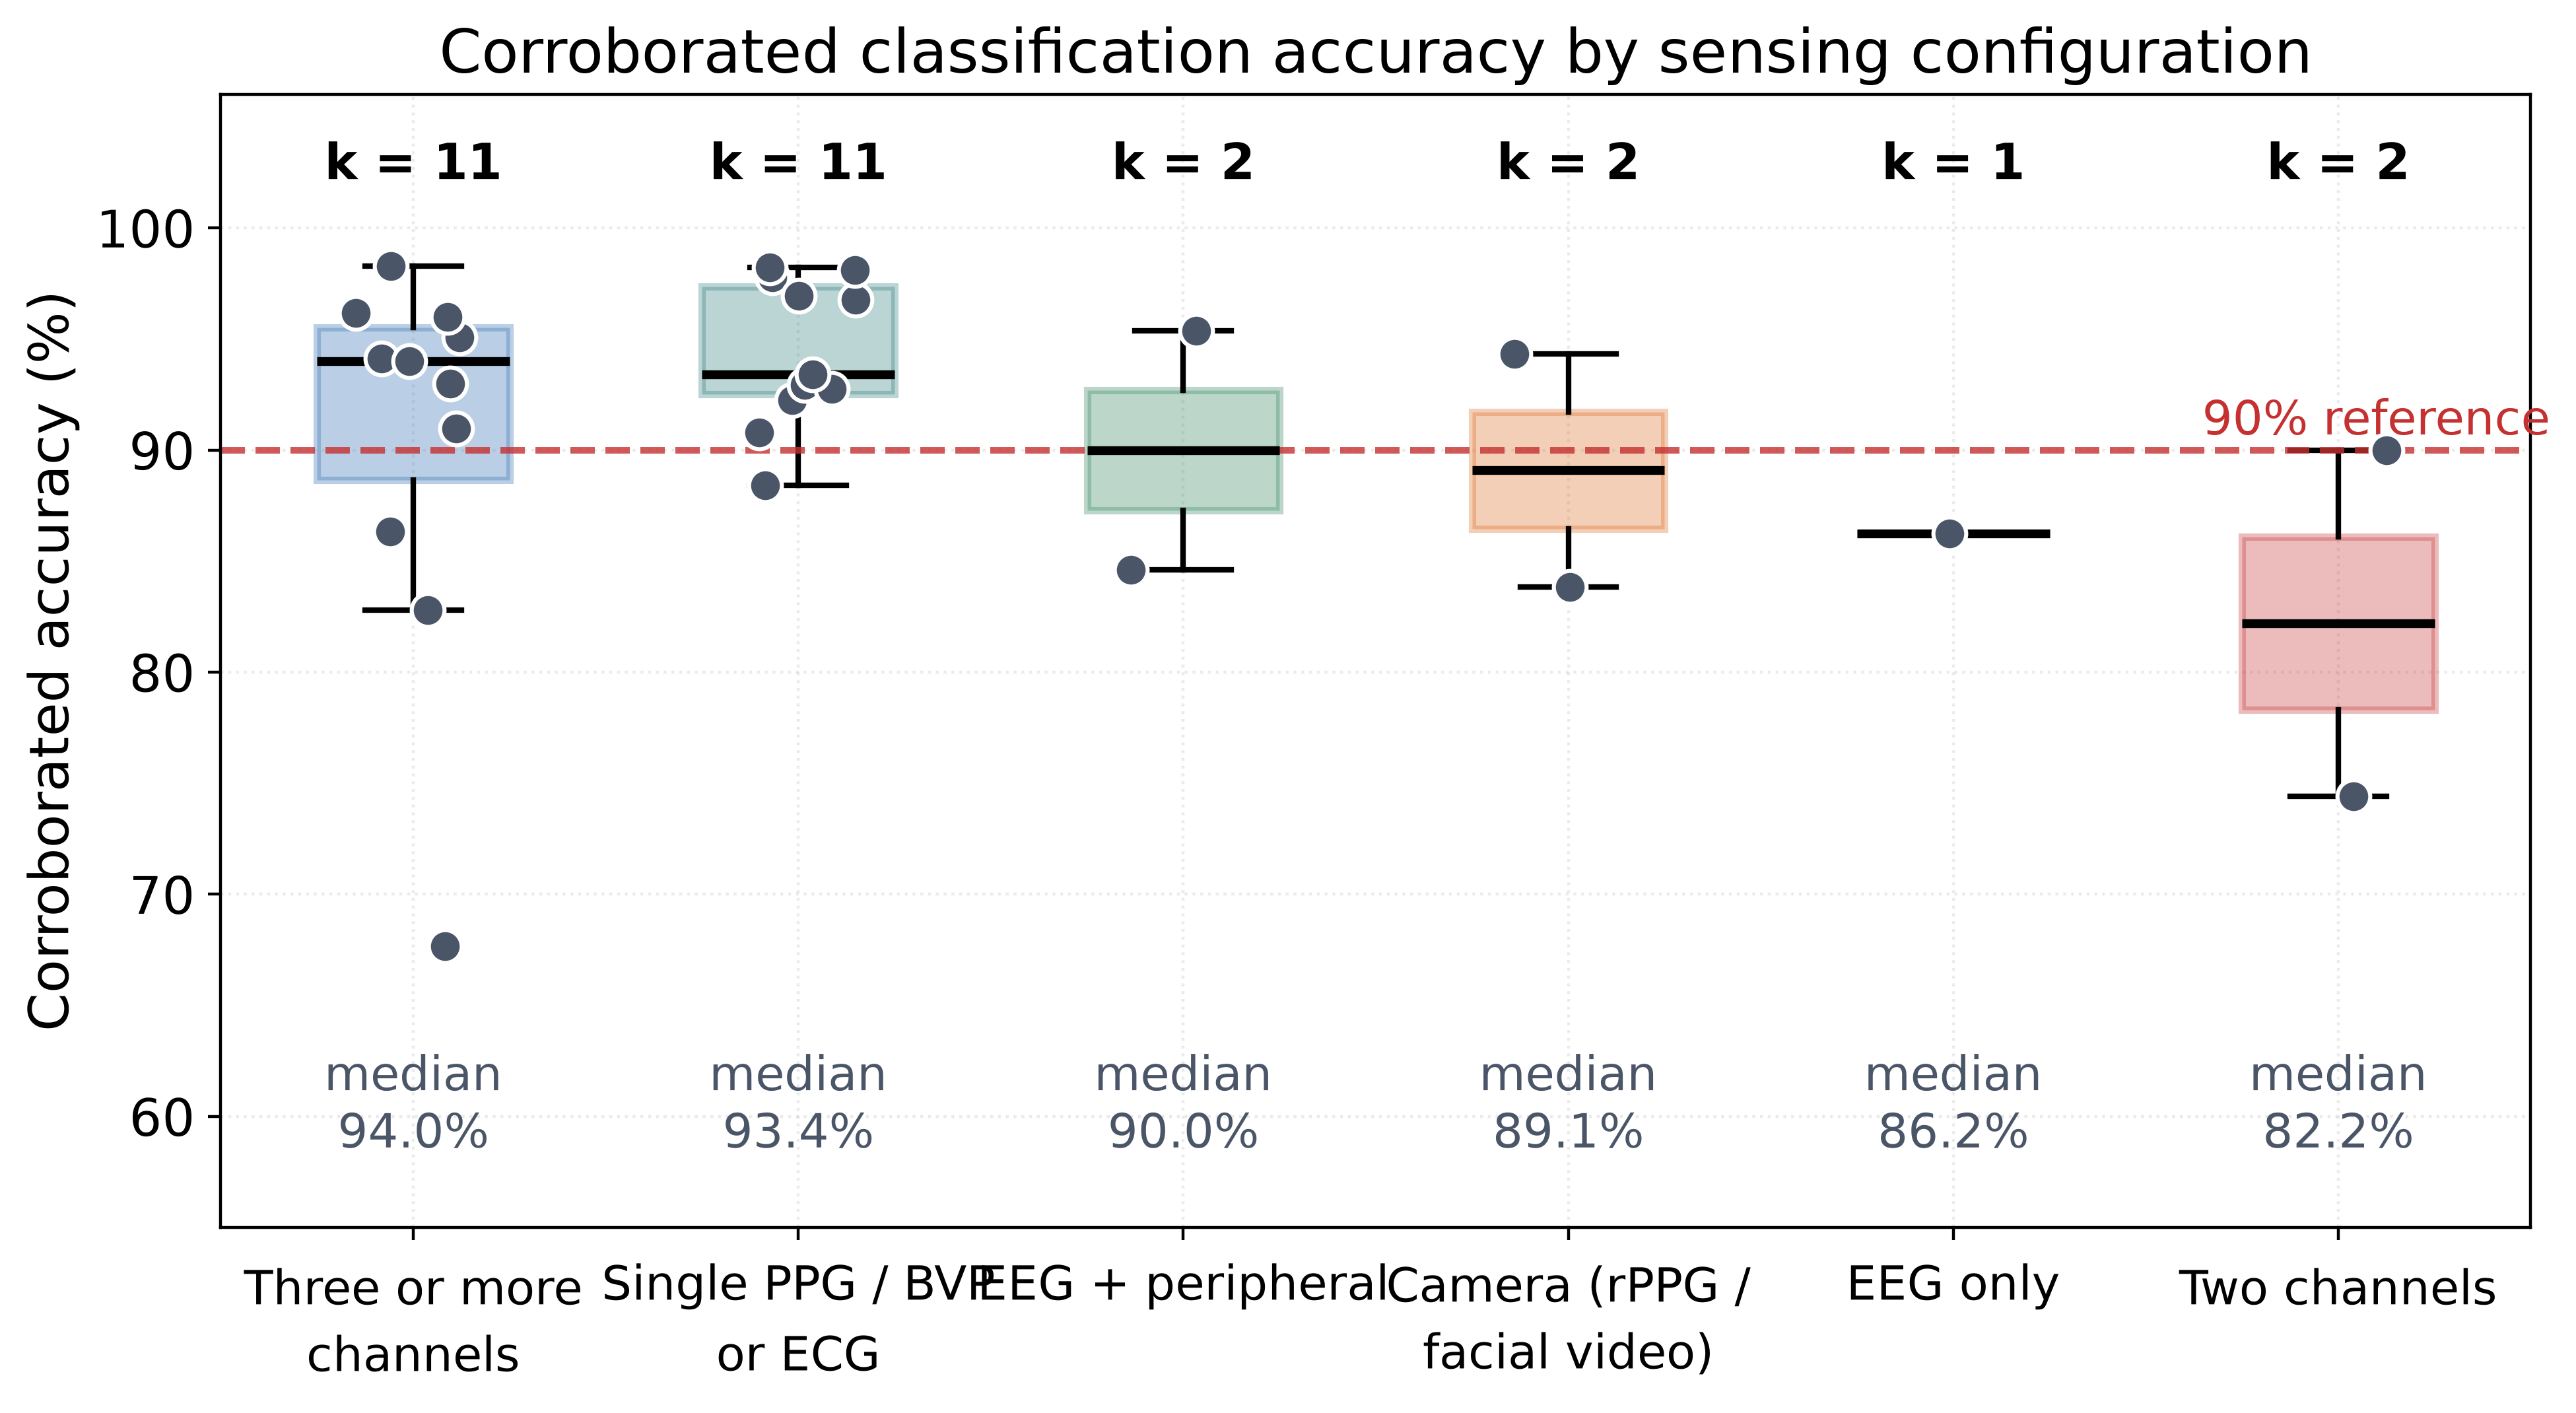
\includegraphics[width=\textwidth]{../figures/fig5_modality.png}
\caption{Corroborated classification accuracy grouped by sensing configuration. Boxes show
the median and interquartile range, individual records are overlaid, and the number of
records $k$ and the group median are annotated. The distributions overlap across
configurations, including between single-channel and three-or-more-channel systems.}
\label{fig:modality}
\end{figure}

\subsubsection{Studies Retained in the Narrative Synthesis}
Thirty-two included studies contribute no numbers because their headline outcome could not be
recovered from the openly retrievable record, yet they define the methodological landscape
that the quantitative findings must be read against. Four themes recur.

\textbf{Architectural elaboration:} Hybrid and generative designs dominate recent output.
A hybrid CNN-transformer with copula-GAN augmentation and Monte Carlo dropout for uncertainty
quantification was evaluated on heart rate and respiratory rate from 34 participants
\cite{r91}; a hybrid CNN-MLP was applied to multi-channel physiological input \cite{r87};
a transformer was applied to five physiological channels from 14 pilots \cite{r42}; a
conditional GAN was used to synthesize physiological time series to address label scarcity
\cite{r70}; and a time-series foundation model was fine-tuned for continuous, explainable
stress monitoring from a wristband \cite{r105}. A study explicitly framed around the
complexity-intrusiveness trade-off compared classical and deep models against how much
daily-life intrusion each device requires \cite{r34}, which is the design question this
review's findings bear on most directly.

\textbf{Deployment constraints:} Several studies target the constraints that matter for
translation rather than accuracy alone. Cost-aware feature selection traded prediction power
against energy, reducing energy cost by up to $94.37\%$ while retaining $90.98\%$ accuracy
\cite{r54}; context-aware selective fusion achieved $2.2\times$ and $2.7\times$ energy
efficiency over conventional fusion on the same hardware \cite{r58}; federated learning was
used to keep wrist EDA on-device \cite{r72}; and secure cloud-connected frameworks were
developed for clinical populations \cite{r51}. Explainability appears both as SHAP and LIME
attribution over deep models \cite{r22} and as genetic-algorithm feature reduction with
Bayesian hyperparameter optimization \cite{r53}.

\textbf{Measurement validity:} A smaller group interrogates whether the signals mean what they
are assumed to mean. Multi-wavelength PPG was validated against microneurography as a
surrogate for stress-induced sympathetic activation \cite{r86}; the relative contribution of
ECG, respiration, GSR and PPG to the stress response was assessed feature by feature, with at
least two statistically significant features recovered from each channel \cite{r29}; salivary
cortisol was used as the reference standard for a context-aware digital biomarker in older
adults \cite{r73}; and rule-based individualised processing of EDA and skin temperature was
proposed in place of a learned model \cite{r48}. Others characterize instrumentation, from
flexible single-lead cardiac electrodes \cite{r76} to multi-parameter assessment platforms
\cite{r41} and wearable bands combining PPG-derived heart rate with GSR \cite{r24}.

\textbf{Generalization as an explicit target:} Three studies treat transfer as the object of
study rather than a limitation. An ensemble of gradient boosting and a neural network trained
on a synthesized 200-subject corpus pooled from SWELL, NEURO, WESAD and UBFC-Phys reported
$25\%$ better predictive performance than singular models, with data and code released
publicly \cite{r101}. Subject-specific baseline normalization against resting state supported
$90.8\%$ accuracy under LOSO validation \cite{r21}. Sleep data from a consumer ring was used
to predict perceived stress longitudinally in first-year students, an outcome regime in which
the achievable performance is far below laboratory figures \cite{r102}. These are the studies
whose design most closely anticipates the conclusions drawn in Sections~4.3 and~4.4.

\subsection{Benchmark Saturation}
WESAD is the reference dataset of this literature and supplies 10 of the 34 corroborated
outcome records. Figure~\ref{fig:wesad} examines what those records actually discriminate.
Figure~\ref{fig:wesad}(a) ranks every corroborated WESAD result by accuracy and colors each
by validation protocol; Figure~\ref{fig:wesad}(b) stratifies the same records by protocol.

Excluding the single subject-independent generalized evaluation, 9 records span
$86.34\%$ to $98.23\%$ and 7 of those 9 exceed $92\%$. That band is occupied indiscriminately
by a context-aware wrist ensemble \cite{r58}, a capsule network on HRV features \cite{r61}, a
$k$-nearest-neighbour classifier on 65 handcrafted features \cite{r14}, a residual
transformer on blood volume pulse \cite{r50} and a transpose-enhanced autoencoder \cite{r55}.
A classical KNN pipeline at $96.00\%$ \cite{r14} is not meaningfully separated from a
transformer at $98.23\%$ \cite{r50}. When architectures spanning two decades of methodological
development are compressed into two percentage points, the benchmark is no longer measuring
architecture.

Figure~\ref{fig:wesad}(b) makes the more consequential point. The median of the records whose
protocol was never stated is $95.06\%$, and the median of the records explicitly validated
leave-one-subject-out is $94.59\%$. These are indistinguishable, which means protocol
reporting on WESAD currently carries almost no information. The single record evaluated as a
subject-independent generalized model falls to $67.65\%$ \cite{r33}, more than 27 pp below
every other record on the same dataset. The saturation is therefore not uniform: WESAD is
saturated for subject-dependent and LOSO evaluation and remains far from saturated for
genuine subject-independent generalization, which is the regime relevant to deployment and
the one almost nobody reports.

\begin{figure}[!htbp]
\centering
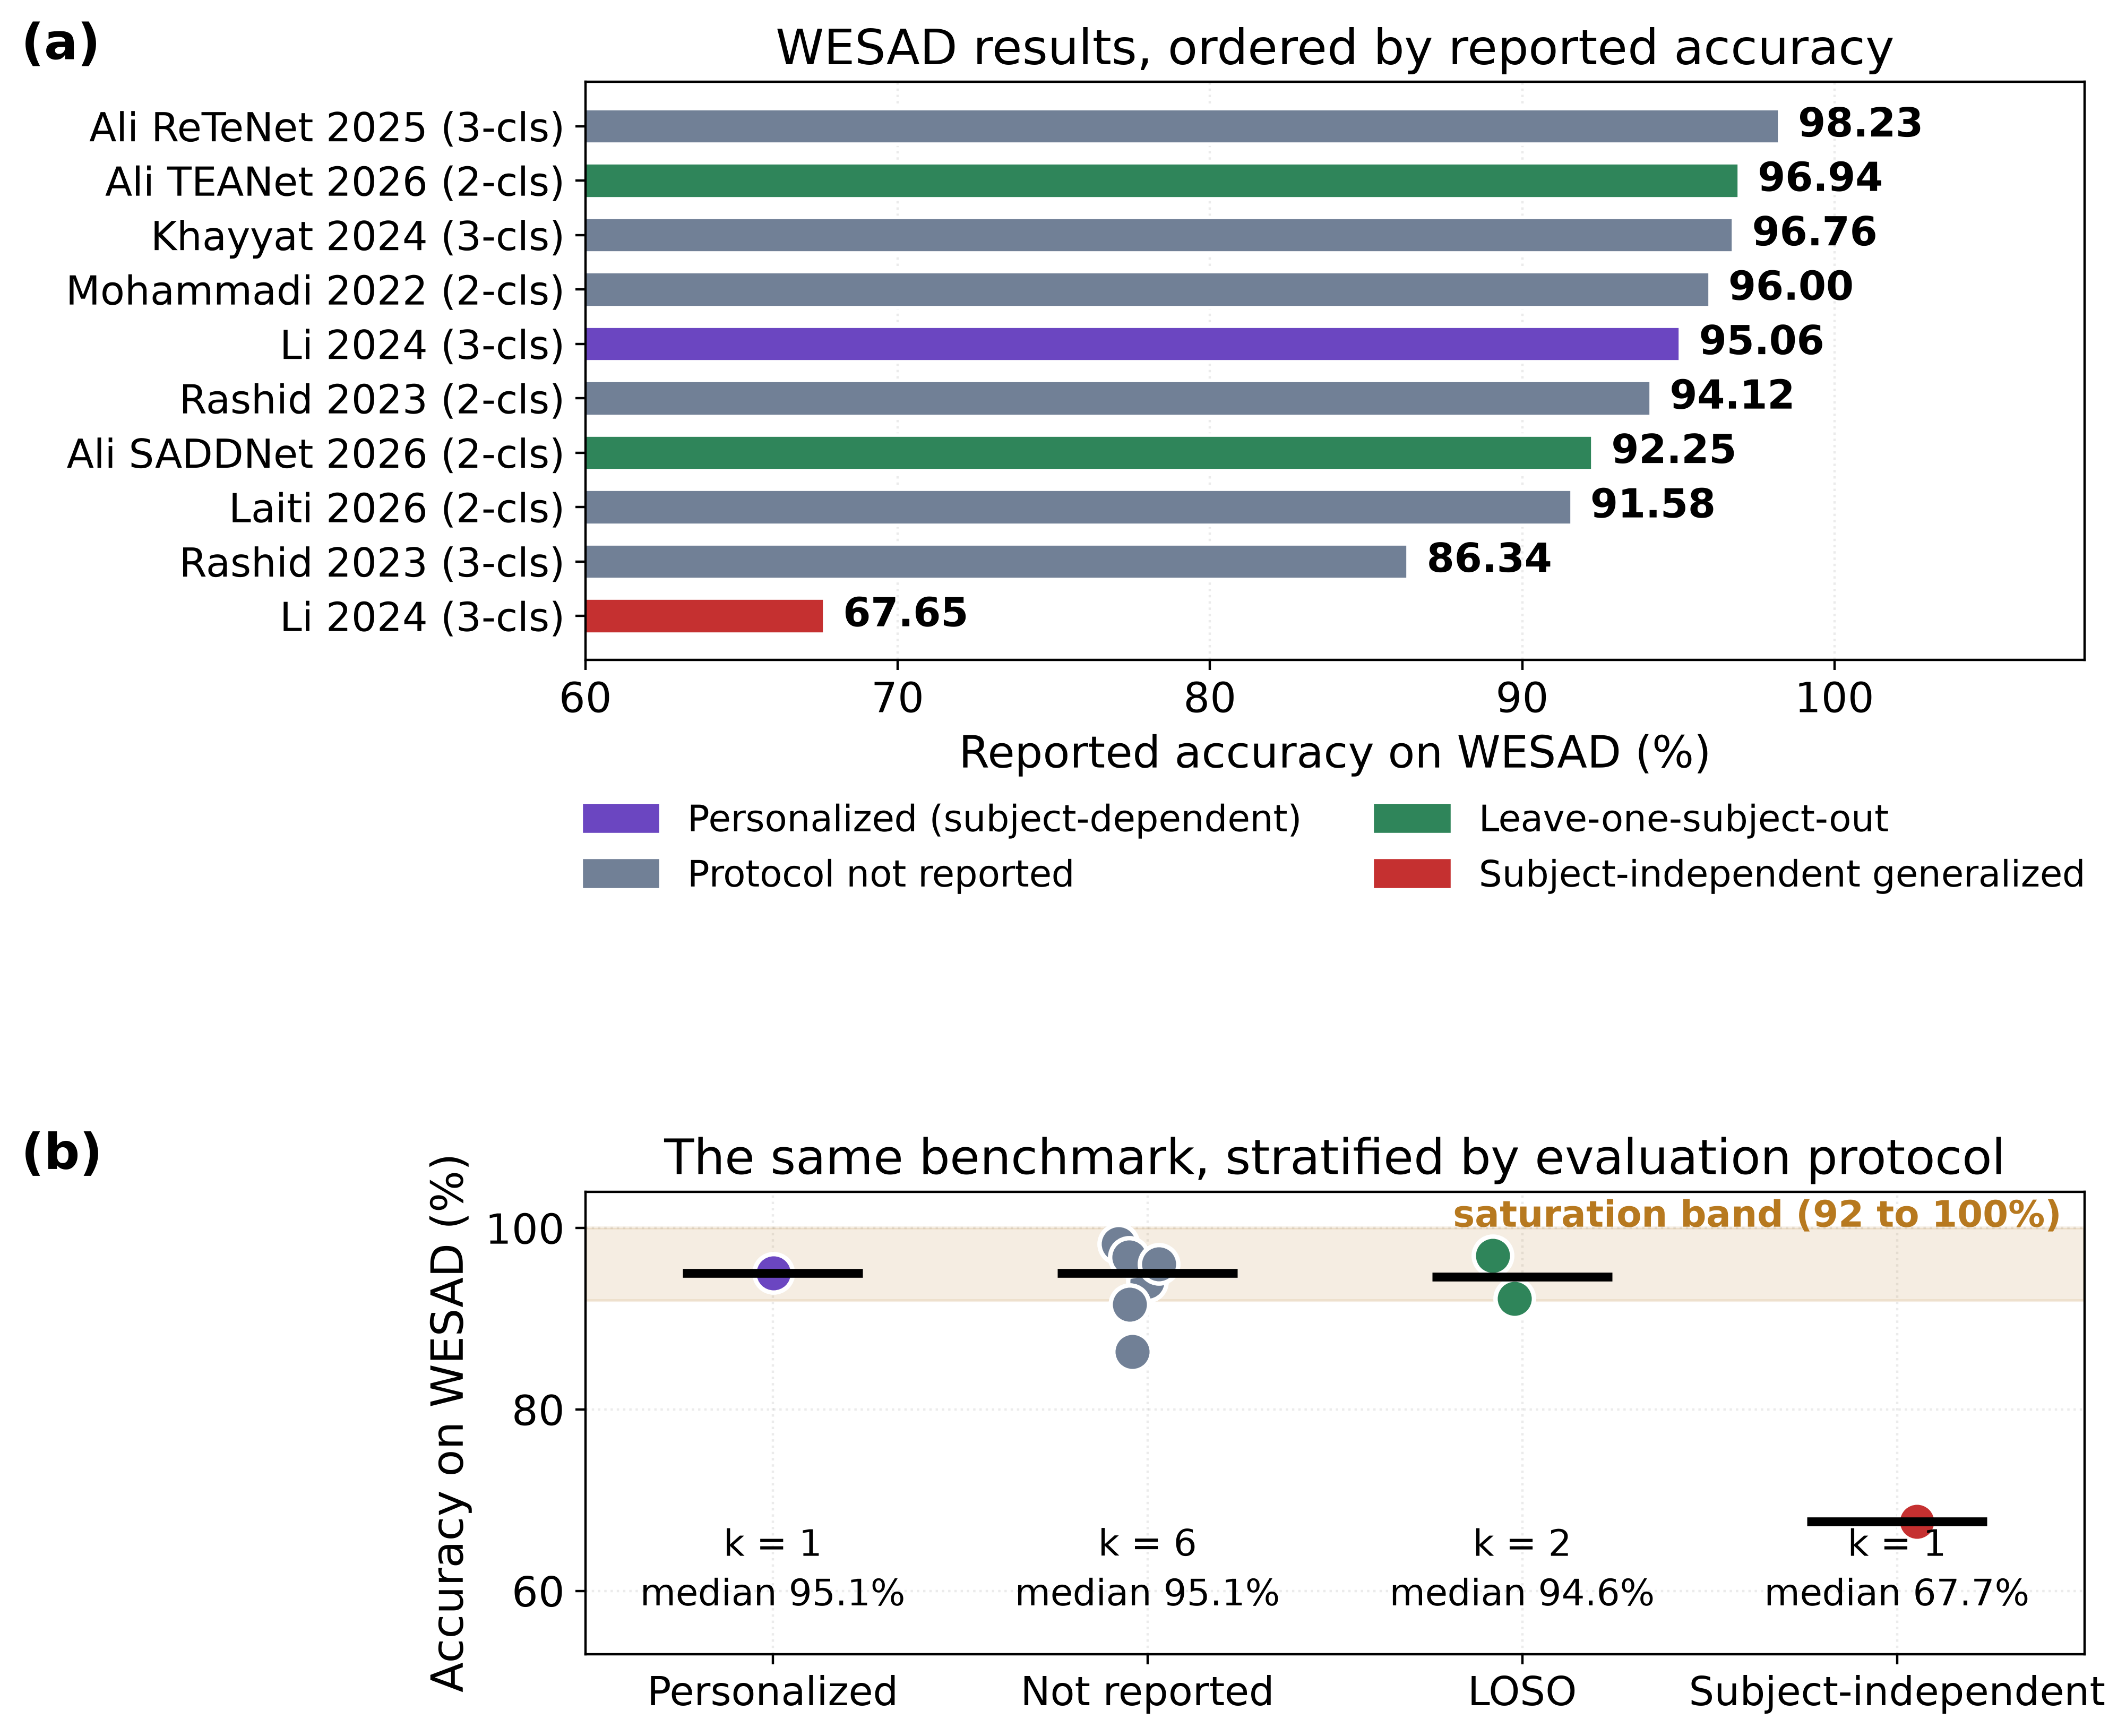
\includegraphics[width=\textwidth]{../figures/fig6_wesad.png}
\caption{Saturation of the WESAD benchmark. Figure~\ref{fig:wesad}(a) ranks all corroborated
WESAD records by reported accuracy, with each bar colored by the validation protocol and the
number of classes given in the label. Figure~\ref{fig:wesad}(b) stratifies the same records by
protocol, showing individual records, the group median as a horizontal rule, and the
saturation band between 92 and 100\%. Personalized and protocol-unreported records are
indistinguishable from leave-one-subject-out records, while the single subject-independent
generalized evaluation falls far below all of them.}
\label{fig:wesad}
\end{figure}

\subsection{Within-Study Fusion Gain}
Four studies in the corpus report a single-modality baseline and a multimodal result on the
same cohort, with the same pipeline and under the same validation protocol.
Table~\ref{tab:t5} gives these contrasts and Figure~\ref{fig:fusion} displays them.

\begin{table}[!htbp]
\centering
\caption{Within-study, protocol-matched contrasts between the best single modality and the
multimodal configuration. Each row holds cohort, pipeline and validation protocol fixed, so
the difference is attributable to the added modality. Gains in the AUROC row are expressed in
percentage points of AUROC and are not pooled with the accuracy rows.}
\label{tab:t5}
\small
\resizebox{\textwidth}{!}{\begin{tabular}{L{3.2cm} L{2.25cm} L{2.8cm} L{1.9cm} C{0.7cm} C{1.4cm} C{1.4cm} C{1.3cm}}
\toprule
\textbf{Study} & \textbf{Single modality} & \textbf{Multimodal configuration} & \textbf{Fusion level} & \textbf{$n$} & \textbf{Unimodal} & \textbf{Multimodal} & \textbf{Gain (pp)} \\
\midrule
Abdul Kader et al. \cite{r75} & EEG & EEG+GSR & Feature-level & 20 & 70.30 & 84.60 & $+$14.30 \\
Campanella et al. \cite{r12} & PPG (HR) & PPG+EDA & Feature-level & 29 & 83.89 & 90.00 & $+$6.11 \\
Awada et al. \cite{r26} & Physiological & Physiological + behavioral & Decision-level & NR & 79.55 & 82.78 & $+$3.23 \\
Kim et al. \cite{r37} & GSR & EEG+GSR & Feature-level & 30 & 94.40 & 95.40 & $+$1.00 \\
\midrule
\multicolumn{7}{l}{\textbf{Median gain} (range 1.00 to 14.30, $k=4$)} & \textbf{$+$4.67} \\
\bottomrule
\end{tabular}}
\end{table}

\begin{figure}[!htbp]
\centering
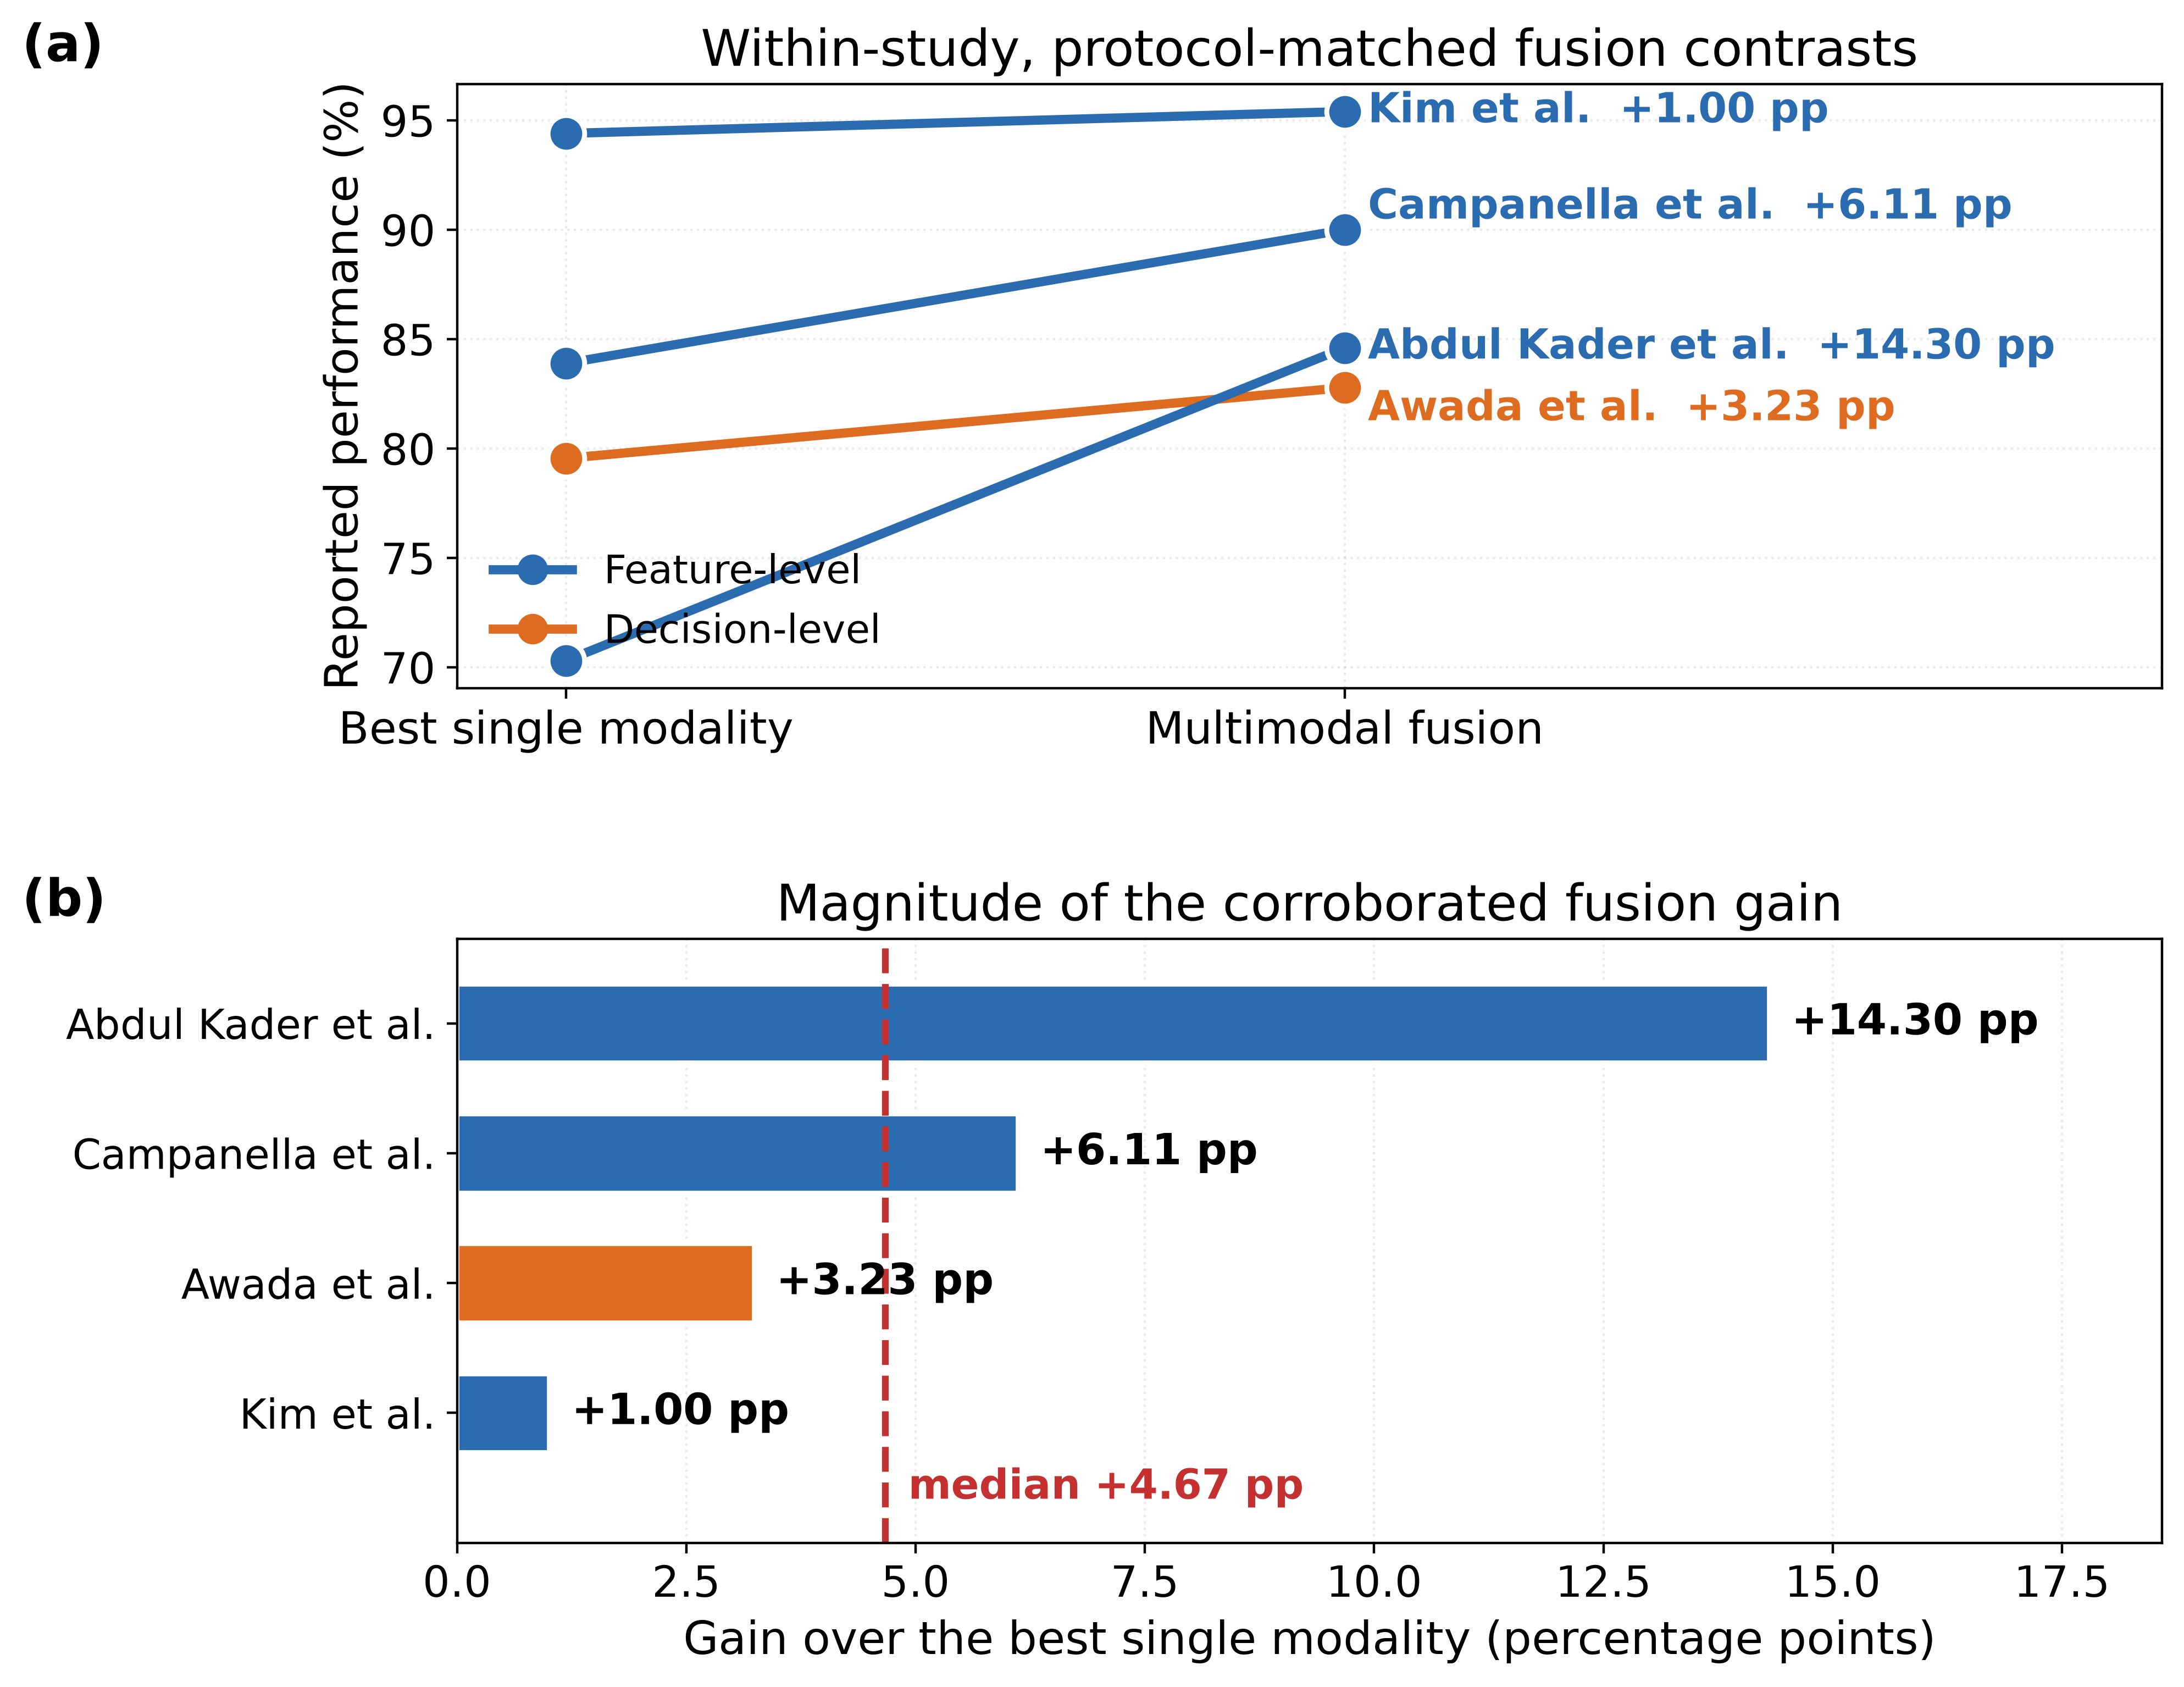
\includegraphics[width=\textwidth]{../figures/fig7_fusion.png}
\caption{Within-study fusion gain. Figure~\ref{fig:fusion}(a) shows each study as a line
connecting its best single-modality result to its multimodal result under an identical
protocol, colored by fusion level. Figure~\ref{fig:fusion}(b) shows the magnitude of each
gain against the median across the four contrasts.}
\label{fig:fusion}
\end{figure}

Every contrast is positive, so fusion does help. The magnitude, however, is modest and highly
uneven. The median gain is $+4.67$ pp, and the range spans $+1.00$ to $+14.30$ pp. The
largest gain, $+14.30$ pp, comes from adding galvanic skin response to a single EEG channel
\cite{r75}, where the baseline modality is weak at $70.30\%$ and the added channel is
physiologically distinct. The smallest, $+1.00$ pp of AUROC, comes from adding EEG to GSR
\cite{r37}, where the baseline is already strong at $0.944$ and fusion adds little headroom.
Adding facial and behavioral features to a physiological wristband in an office cohort
yields $+3.23$ pp, from $79.55\%$ to $82.78\%$ \cite{r26}; notably, the authors of that study
themselves conclude that the small difference indicates physiological data alone may be
adequate for their task. Adding EDA to heart rate gives $+6.11$ pp \cite{r12}.

A coherent pattern emerges. Fusion gain is largest where the unimodal baseline is weakest and
where the added channel is physiologically non-redundant, and it approaches zero as the
baseline strengthens. This is the behavior expected of a complementary-information effect
operating against a ceiling, and it means that headline fusion gains harvested from
weak-baseline studies do not transfer to systems whose unimodal baseline is already strong.

\subsection{Within-Study Evaluation-Induced Gaps}
Ten within-study contrasts isolate the effect of an evaluation choice while holding the model
and data-generating process fixed. Table~\ref{tab:t6} lists them and
Figure~\ref{fig:protocol} compares them against the fusion gains of Section~4.3 on a common
scale.

\begin{table}[!htbp]
\centering
\caption{Within-study contrasts attributable to evaluation choices. Each row reports the same
model or pipeline under a more favorable and a more realistic evaluation condition. The
final rows give the median gap alongside the median within-study fusion gain for direct
comparison.}
\label{tab:t6}
\small
\resizebox{\textwidth}{!}{\begin{tabular}{L{3.1cm} L{4.35cm} L{2.35cm} C{1.2cm} C{1.4cm} C{1.4cm} C{1.3cm}}
\toprule
\textbf{Study} & \textbf{Contrast} & \textbf{Source of the difference} & \textbf{Metric} & \textbf{Favourable} & \textbf{Realistic} & \textbf{Gap (pp)} \\
\midrule
Li \& Washington \cite{r33} & Personalized vs subject-independent & Personalization & F1 & 91.71 & 43.05 & 48.66 \\
Li \& Washington \cite{r33} & Personalized vs subject-independent & Personalization & Accuracy & 95.06 & 67.65 & 27.41 \\
Laiti et al. \cite{r49} & WESAD vs Wellby real-world cohort & Dataset transfer & AUROC & 91.58 & 77.02 & 14.56 \\
Toshnazarov et al. \cite{r13} & Laboratory vs free-living & Deployment setting & F1 & 84.00 & 71.00 & 13.00 \\
Xu et al. \cite{r16} & Stress state vs stress level & Task granularity & Accuracy & 94.33 & 83.83 & 10.50 \\
Rashid et al. \cite{r58} & Binary vs three-class & Task granularity & Accuracy & 94.12 & 86.34 & 7.78 \\
Ali et al. \cite{r55} & WESAD vs in-house cohort & Dataset transfer & Accuracy & 96.94 & 92.94 & 4.00 \\
Khayyat et al. \cite{r61} & WESAD vs SWELL-KW & Dataset transfer & Accuracy & 96.76 & 92.76 & 4.00 \\
Khayyat et al. \cite{r61} & Binary vs multiclass (WESAD) & Task granularity & Accuracy & 99.82 & 96.76 & 3.06 \\
Shikha et al. \cite{r53} & Two-level vs three-level stress & Task granularity & Accuracy & 98.28 & 97.02 & 1.26 \\
\midrule
\multicolumn{6}{l}{\textbf{Median evaluation-induced gap} (range 1.26 to 48.66, $k=10$)} & \textbf{9.14} \\
\multicolumn{6}{l}{Median within-study fusion gain for comparison ($k=4$)} & 4.67 \\
\bottomrule
\end{tabular}}
\end{table}

\begin{figure}[!htbp]
\centering
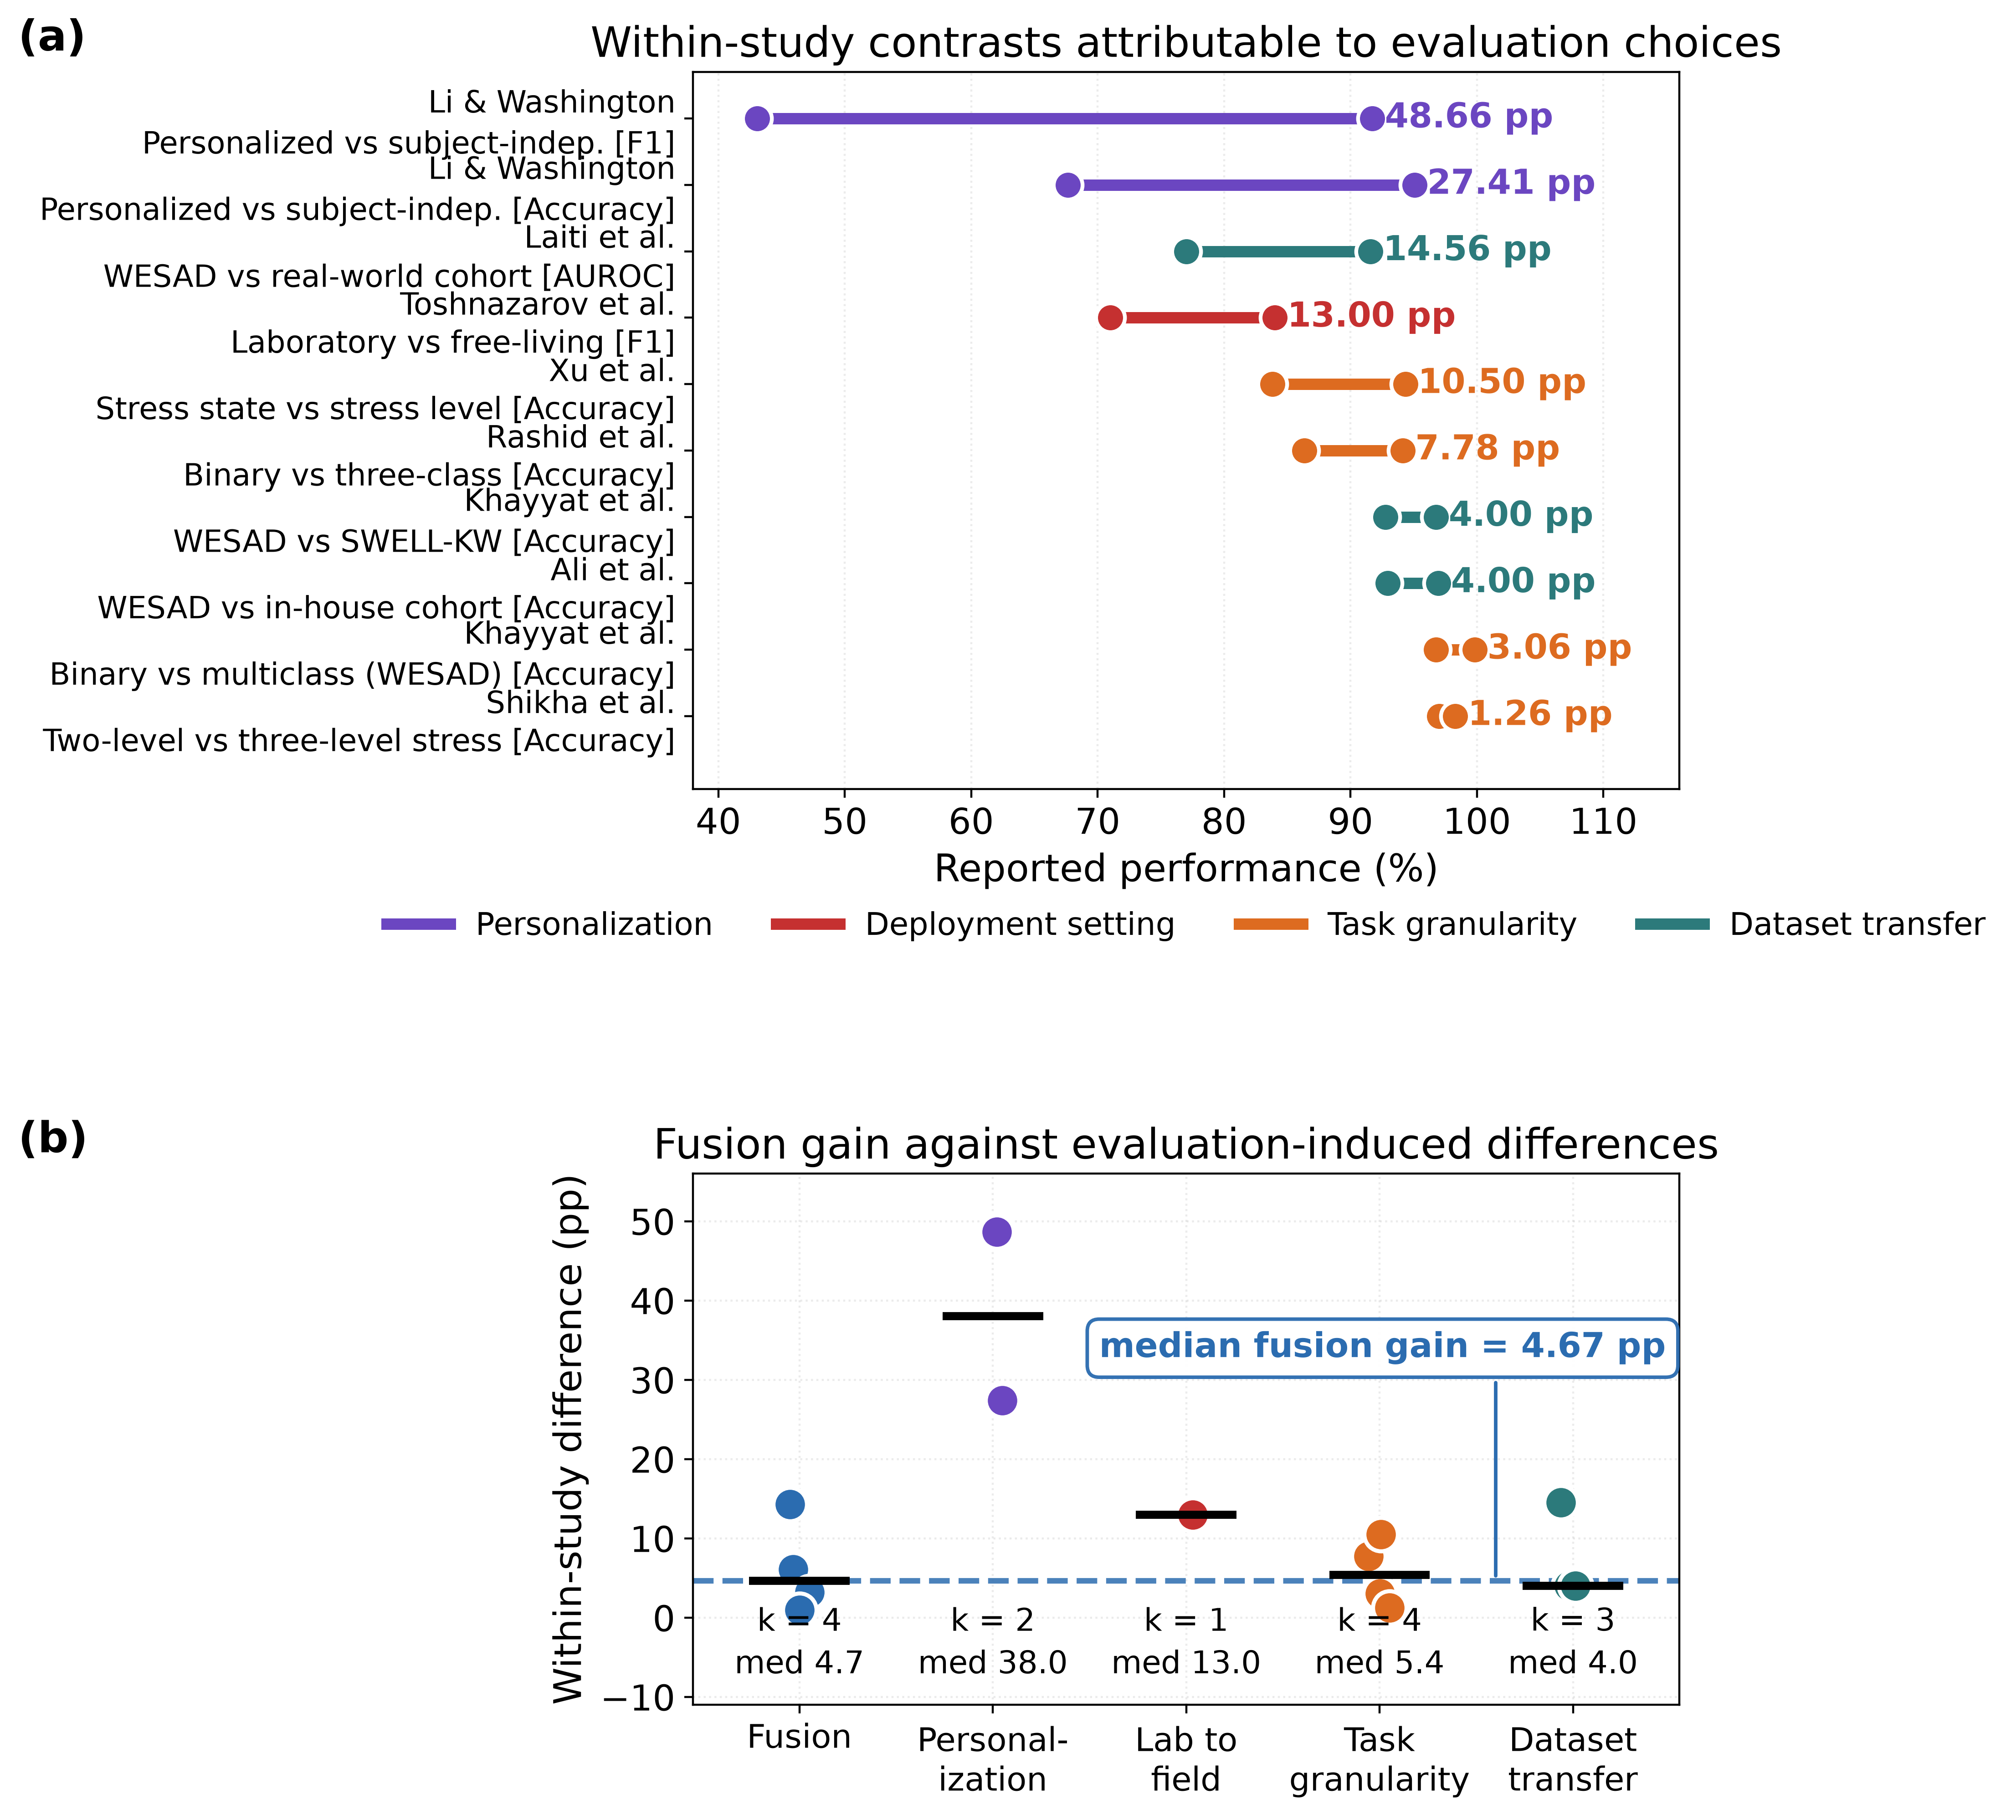
\includegraphics[width=\textwidth]{../figures/fig8_protocol_vs_fusion.png}
\caption{Evaluation effects against fusion effects. Figure~\ref{fig:protocol}(a) shows each
within-study evaluation contrast as a segment joining the favorable and the realistic
condition, colored by the source of the difference and annotated with the gap in percentage
points. Figure~\ref{fig:protocol}(b) places the four within-study fusion gains and the four
families of evaluation contrast on a common axis, with group medians shown as horizontal
rules and the median fusion gain marked by the dashed line.}
\label{fig:protocol}
\end{figure}

The median evaluation-induced gap is $9.14$ pp, approximately twice the median fusion gain of
$4.67$ pp, and the four families differ sharply in severity.

\textbf{Personalization:} This is the dominant effect in the corpus, with a median gap of
$38.03$ pp. In a single study using consumer wearable data for three-class affect
classification, a personalized model reached $95.06\%$ accuracy with an F1 of $91.71$, while
the subject-exclusive generalized model on the same data reached $67.65\%$ with an F1 of
$43.05$ \cite{r33}. The accuracy gap of $27.41$ pp is $5.9$ times the median fusion gain, and
the F1 gap of $48.66$ pp is $10.4$ times it. The F1 collapse is the more diagnostic figure:
it indicates that the generalized model is not merely less accurate but is failing on the
minority classes that matter, which an accuracy figure partially conceals.

\textbf{Deployment setting:} Moving from controlled laboratory recording to free living cost
$13.00$ pp of F1 in a smartwatch study that evaluated both, falling from $0.84$ to $0.71$
\cite{r13}. That single study is worth more for deployment planning than any number of
laboratory accuracy figures, and it is nearly three times the median fusion gain.

\textbf{Dataset transfer:} Three contrasts give a median of $4.00$ pp, but the range is
instructive. Transfer between two curated laboratory benchmarks is cheap: $4.00$ pp between
WESAD and SWELL-KW \cite{r61} and $4.00$ pp between WESAD and an in-house cohort under
matched LOSO validation \cite{r55}. Transfer from a benchmark to a genuine real-world student
cohort is not: AUROC fell from $91.58$ on WESAD to $77.02$ in a real-world deployment, a gap
of $14.56$ pp \cite{r49}. Benchmark-to-benchmark transfer therefore substantially
underestimates benchmark-to-field transfer, and reporting the former as evidence of
generalization is misleading.

\textbf{Task granularity:} Four contrasts give a median of $5.42$ pp. Binary stress detection
exceeds three-class detection by $7.78$ pp in one wrist-based ensemble \cite{r58}, binary
stress state exceeds graded stress level by $10.50$ pp in a facial video system \cite{r16},
and smaller penalties of $3.06$ pp \cite{r61} and $1.26$ pp \cite{r53} appear elsewhere. Since
clinical and operational utility generally requires graded rather than binary output, the
binary figures that dominate the literature systematically overstate deployable performance.

\subsection{Cohort Size, Transfer and Reporting}
Figure~\ref{fig:transfer} examines two further properties of the evidence base.
Figure~\ref{fig:transfer}(a) shows the three contrasts in which a model was evaluated both on
its development condition and on a transfer condition. Figure~\ref{fig:transfer}(b) plots
corroborated accuracy against evaluation cohort size on a logarithmic axis.

\begin{figure}[!htbp]
\centering
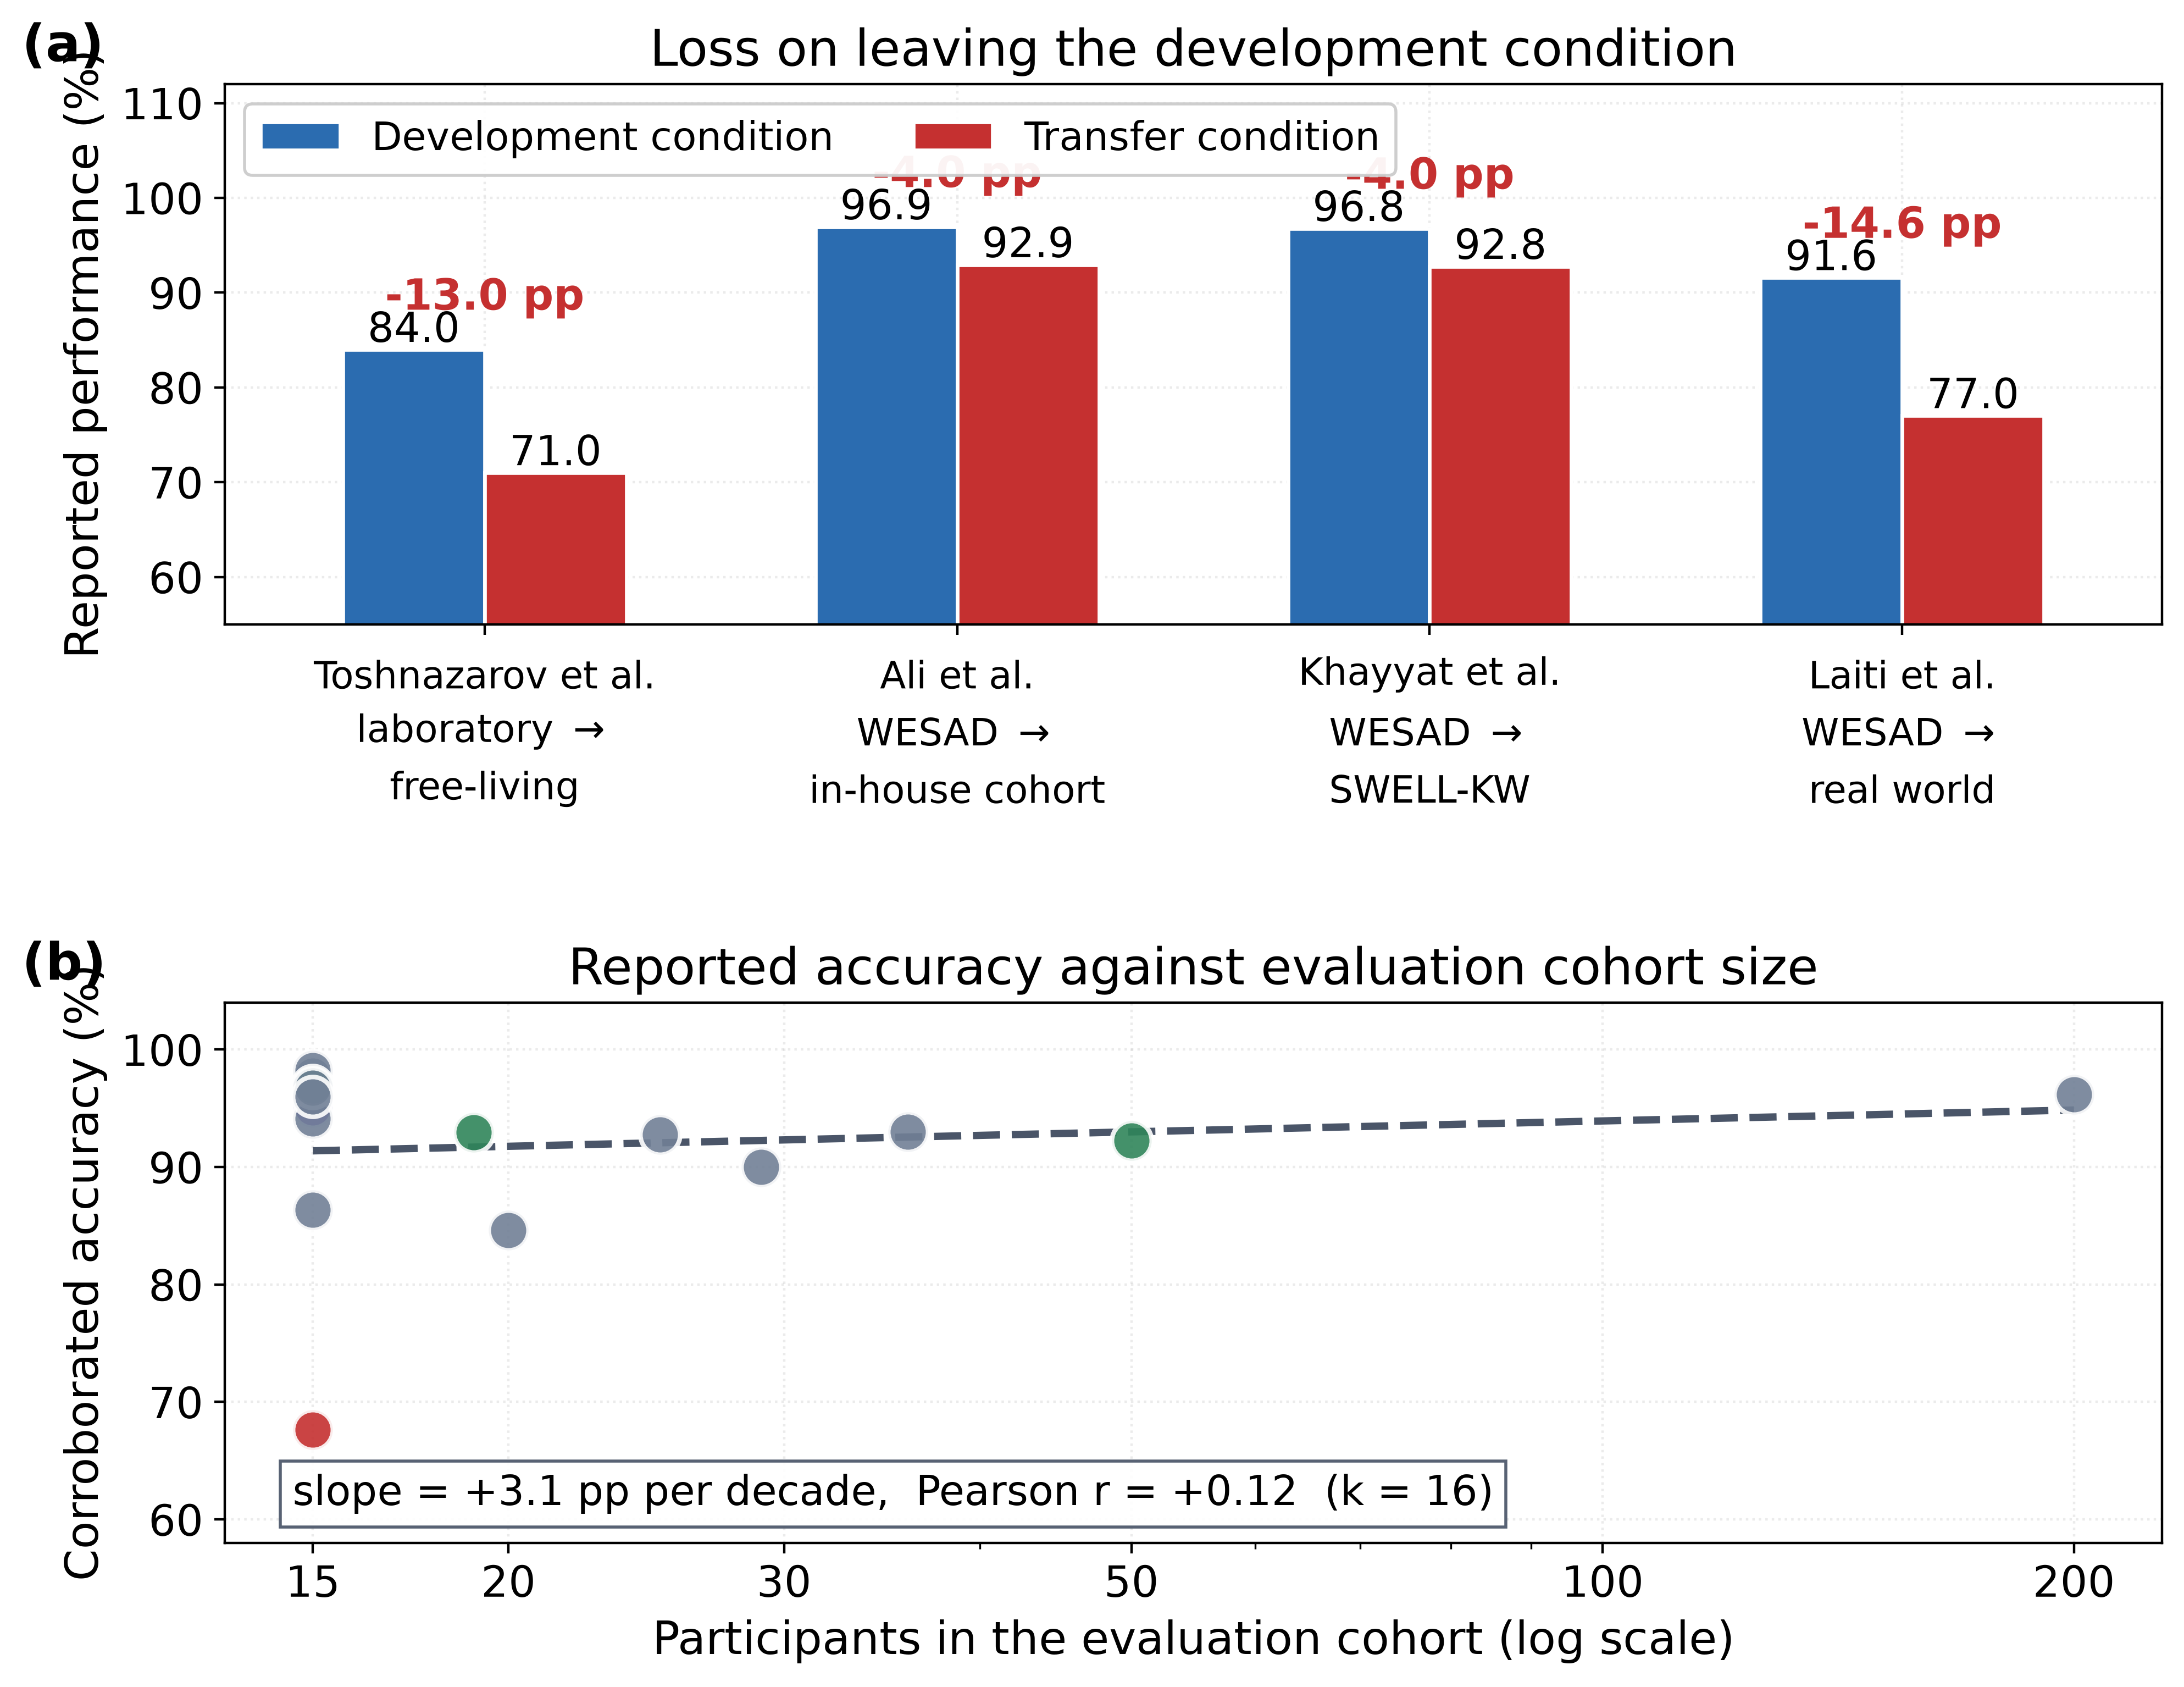
\includegraphics[width=\textwidth]{../figures/fig9_transfer.png}
\caption{Transfer behavior and the absence of a cohort-size effect.
Figure~\ref{fig:transfer}(a) contrasts performance on the development condition with
performance on the transfer condition for the three studies reporting both, annotated with
the loss in percentage points. Figure~\ref{fig:transfer}(b) plots corroborated accuracy
against the number of participants in the evaluation cohort on a logarithmic axis, with
points colored by validation protocol and a least-squares fit on the log axis.}
\label{fig:transfer}
\end{figure}

The relationship between cohort size and reported accuracy is essentially flat
($r=+0.12$, slope $+3.1$ pp per decade, $k=16$). Studies evaluating on 15 participants report
accuracies indistinguishable from studies evaluating on 200. Under any reasonable model of
task difficulty, a larger and more heterogeneous cohort should be harder, so a flat or
slightly positive relationship is not evidence that small studies are adequate; it is
evidence that reported accuracy is being set by evaluation design rather than by the
difficulty of the underlying problem.

Figure~\ref{fig:verify} reports the verification and reporting audit.
Figure~\ref{fig:verify}(a) shows that a headline outcome could be independently corroborated
for 28 of 60 included studies (46.7\%). Figure~\ref{fig:verify}(b) shows recovery rates for
each reporting item: the evaluation cohort size was recoverable for 18 studies (30.0\%),
whether a public benchmark was used for 14 (23.3\%), the validation protocol for 8 (13.3\%)
and any variance or confidence interval for only 3 (5.0\%).

\begin{figure}[!htbp]
\centering
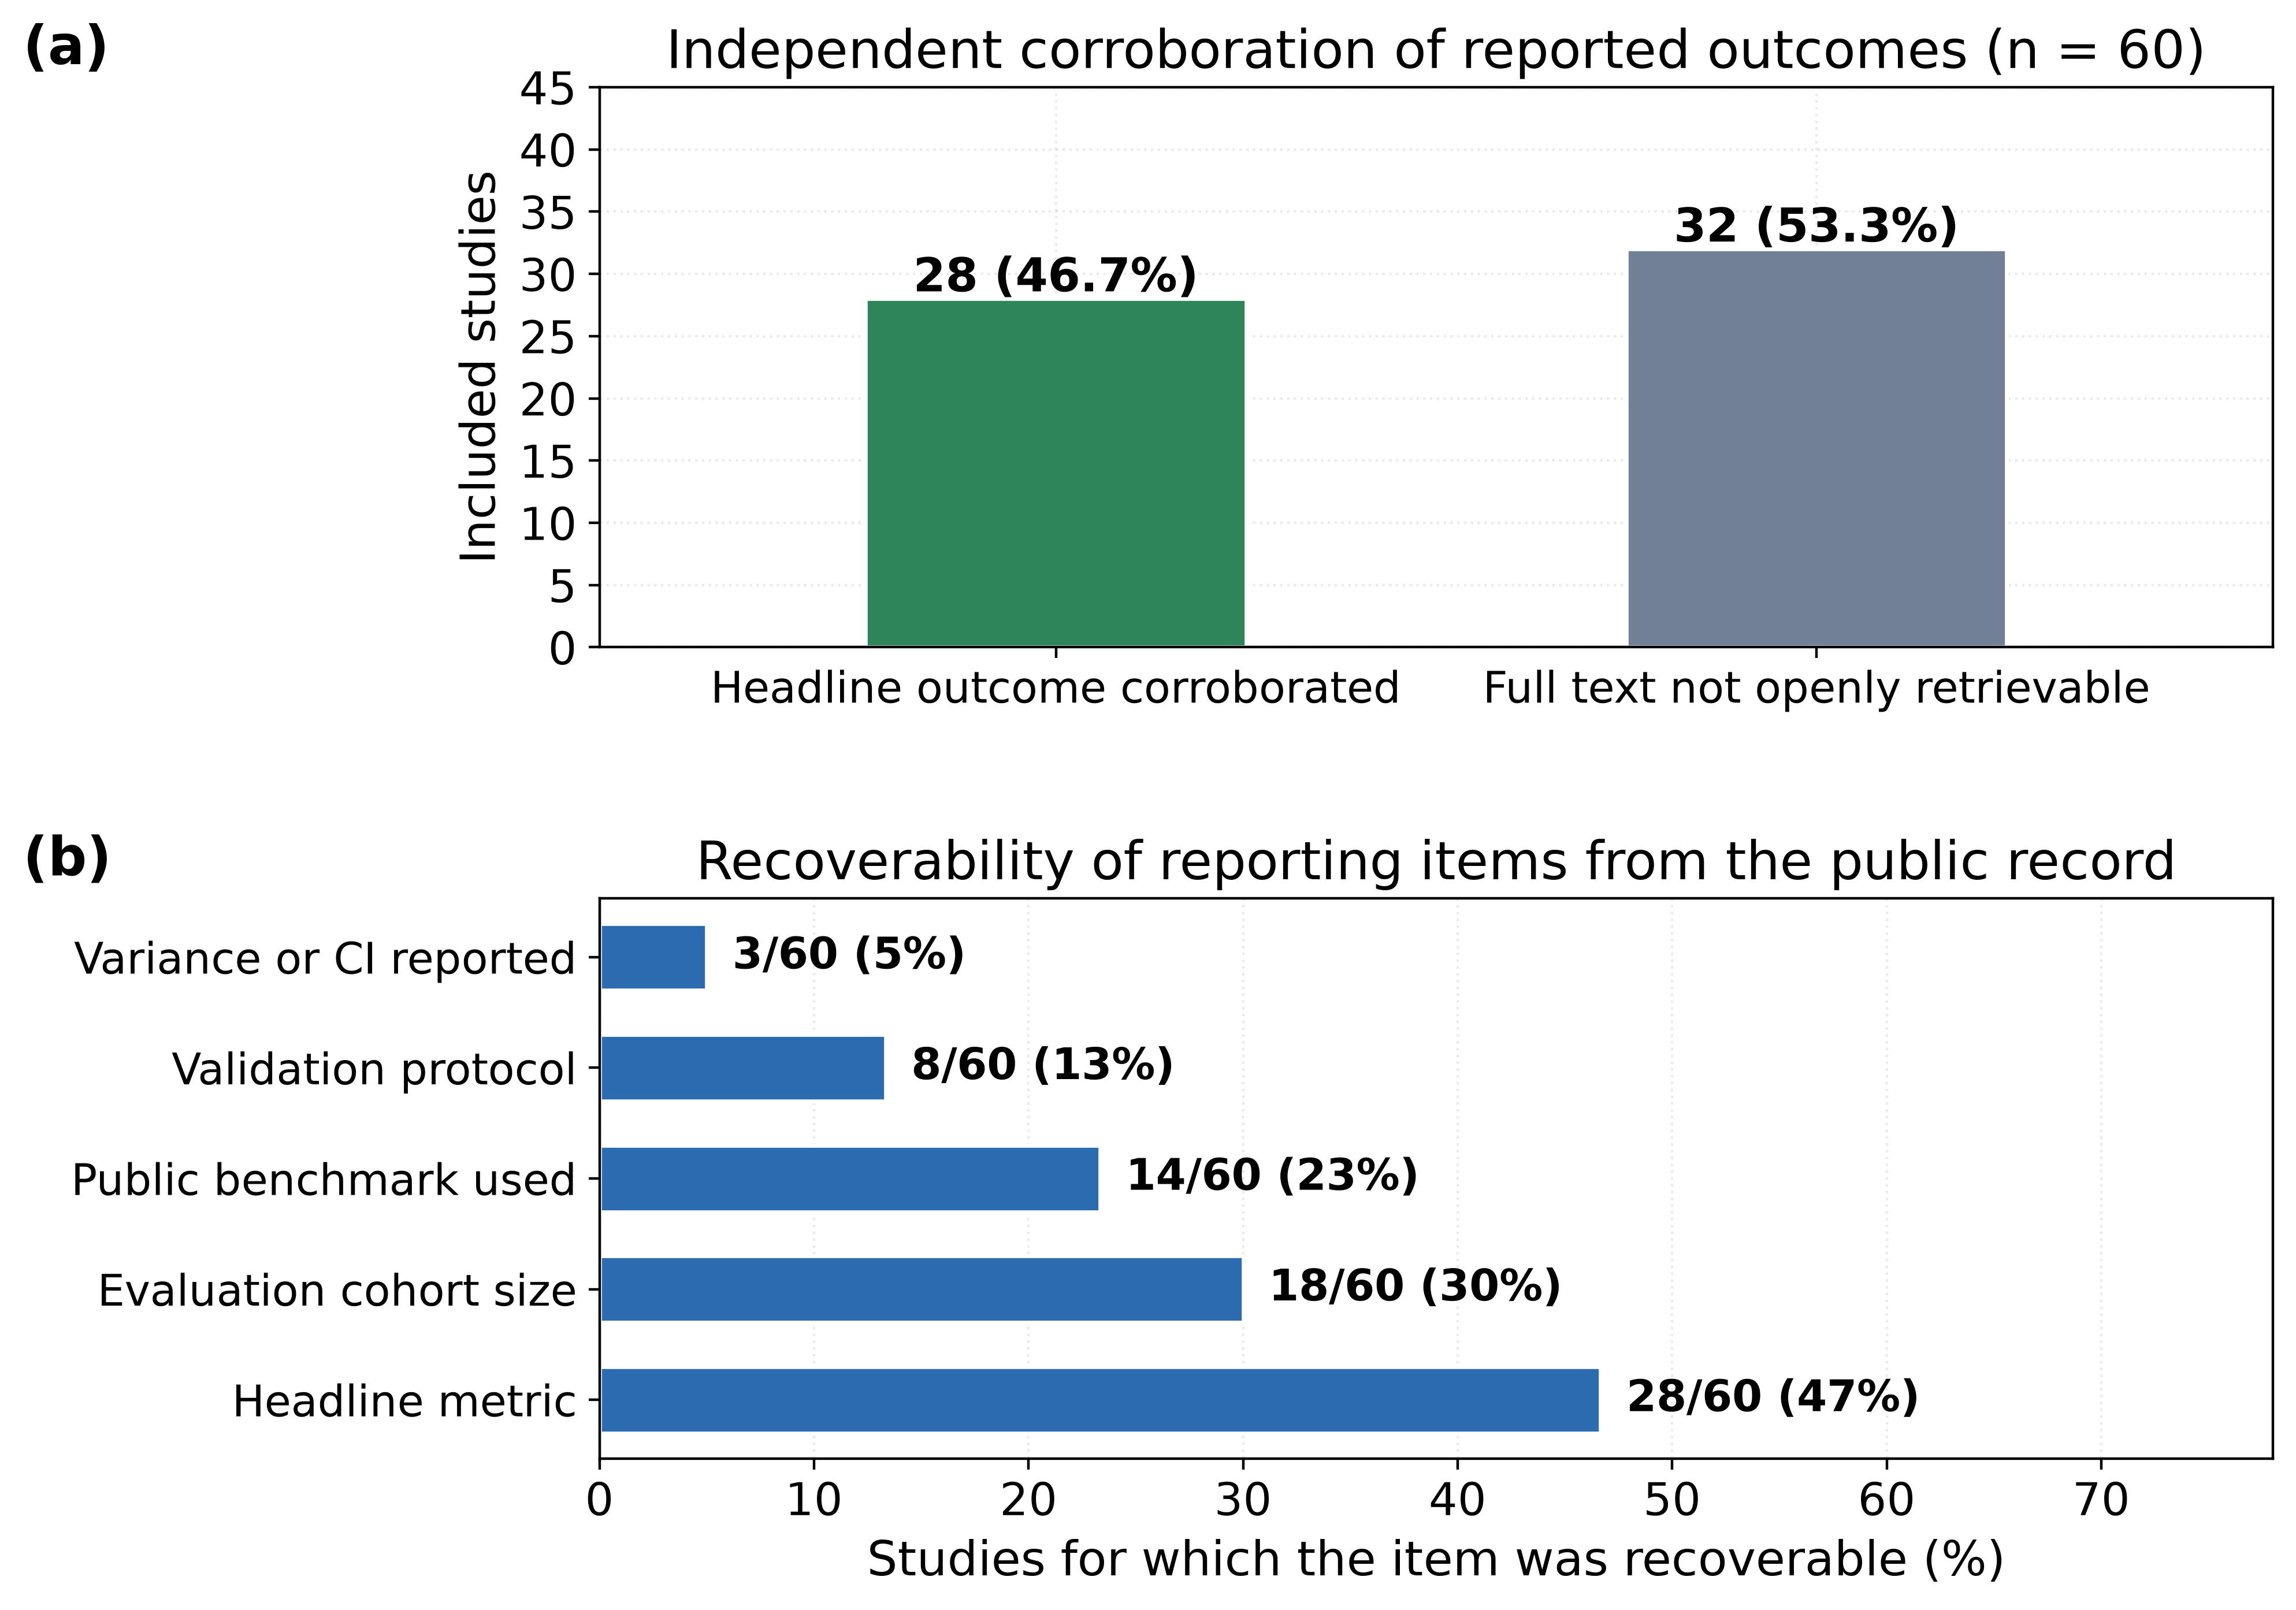
\includegraphics[width=\textwidth]{../figures/fig10_verifiability.png}
\caption{Verification and reporting audit across all 60 included studies.
Figure~\ref{fig:verify}(a) shows the proportion of studies for which a headline outcome could
be independently corroborated from the openly retrievable record.
Figure~\ref{fig:verify}(b) shows the recovery rate for each of the five reporting items,
with the count and percentage annotated.}
\label{fig:verify}
\end{figure}

These rates should be read as a property of the openly retrievable record rather than as a
judgement on the studies, since much of the corpus sits behind subscription access. The
implication is nevertheless concrete and is the central practical finding of
Section~4.4: for roughly seven studies in eight, a reader without subscription access cannot
determine the validation protocol, and therefore cannot determine whether a quoted accuracy
describes subject-dependent or subject-independent performance. Given that this single
distinction is worth up to $27.41$ pp of accuracy and $48.66$ pp of F1 within one study
\cite{r33}, an unlabeled accuracy figure in this literature carries very little information.

\begin{table}[!htbp]
\centering
\caption{Constraints on deployment, the corroborated quantitative evidence for each, and its
implication. Only effects supported by a within-study contrast or a directly corroborated
value are listed; magnitudes are those reported in Tables~\ref{tab:t5} and~\ref{tab:t6}.}
\label{tab:t7}
\small
\resizebox{\textwidth}{!}{%
\begin{tabular}{L{2.9cm} L{5.15cm} C{2.3cm} L{5.35cm}}
\toprule
\textbf{Constraint} & \textbf{Corroborated evidence} & \textbf{Magnitude} &
\textbf{Implication for deployment} \\
\midrule
Subject heterogeneity & Personalized versus subject-exclusive generalized model on identical
  data \cite{r33} & 27.41 pp accuracy; 48.66 pp F1 & Calibration data per user is the single
  highest-value design decision; generalized models must not be specified from personalized
  results. \\
Ecological validity & Laboratory versus free-living F1 in the same smartwatch study
  \cite{r13} & 13.00 pp F1 & Laboratory accuracy is not an upper bound that degrades
  gracefully; field validation is required before any deployment claim. \\
Benchmark-to-field transfer & WESAD AUROC versus real-world student cohort AUROC
  \cite{r49} & 14.56 pp AUROC & Benchmark-to-benchmark transfer (4.00 pp) understates
  benchmark-to-field transfer by roughly a factor of three. \\
Output granularity & Binary versus graded outputs across four studies
  \cite{r16,r53,r58,r61} & 5.42 pp median & Binary benchmarks overstate the performance of
  the graded outputs that clinical and operational use requires. \\
Benchmark saturation & 7 of 9 non-subject-independent WESAD records above 92\%, spanning KNN
  to transformers \cite{r14,r50,r55,r58,r61} & $<$ 2 pp separating classical from
  transformer models & WESAD can no longer adjudicate between architectures; new
  architectural claims need a harder or subject-independent evaluation. \\
Reporting completeness & Validation protocol recoverable for 8 of 60 studies; variance for 3
  of 60 & 13.3\%; 5.0\% & Most reported accuracies cannot be interpreted, and meta-analytic
  pooling across this literature is not currently defensible. \\
Modality redundancy & Fusion gain shrinks as the unimodal baseline strengthens
  \cite{r12,r26,r37,r75} & $+1.00$ to $+14.30$ pp & Sensor count should be justified against
  the specific unimodal baseline, not against a generic fusion benefit. \\
\bottomrule
\end{tabular}}
\end{table}
